\chapter{Análisis y discusión de resultados}
\label{ch:resultados}
\section{Proceso de entrenamiento}\label{sec:analisistrain}
El primer paso para poder verificar la validez del sistema de predicción con la red neuronal es el análisis 
de las curvas de entrenamiento. Se puede extraer información valiosa acerca del rendimiento observando 
la naturaleza de dichas curvas. Se ha trabajado con el conjunto de datos explorado en la Sección(\ref{sec:dataset}) 
que cuenta con un total de 26356 muestras entre datos reales y datos aumentados. Se procede a explorar la naturaleza 
de las curvas de entrenamiento.
    
    \subsection{Análisis de las curvas de entrenamiento}

    Las curvas de entrenamiento representan una herramienta bastante valiosa a la hora de evaluar el proceso de entrenamiento 
    de un algoritmo de aprendizaje. A través de las mismas se puede extraer información sobre la convergencia del entrenamiento, 
    la evolución del mismo y también, gracias al proceso de validación cruzada, se puede analizar la presencia de sobreentrenamiento 
    en el sistema.

        \subsubsection{Error de entrenamiento}

        En la Figura(\ref{fig:trainloss}) se puede observar la evolución del error de entrenamiento para ambas arquitecturas implementadas. 
        %% foto de ejemplo
        \begin{figure}[!ht] 
            \centering
            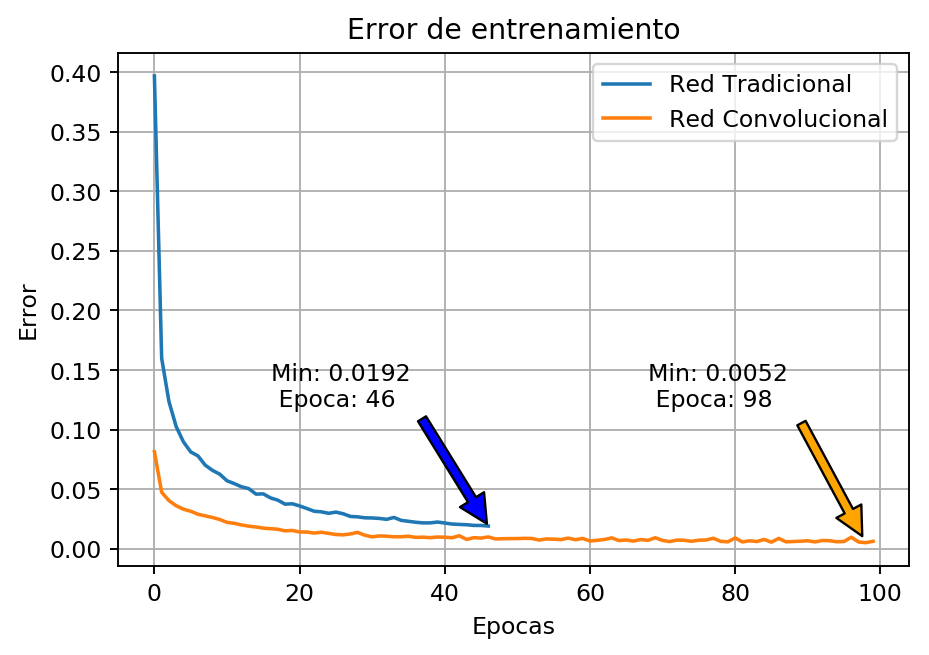
\includegraphics[width=0.75\textwidth]{img/trainloss}
            \caption[Error de entrenamiento]{Error de entrenamiento. Fuente: Elaboración propia. }
            \label{fig:trainloss}
        \end{figure}

        Observando las curvas de error de entrenamiento se pueden realizar las siguientes observaciones con respecto a la red neuronal convolucional:

        \begin{itemize}
            \item \textbf{El error de entrenamiento inicial es menor:} Esto indica que la capacidad de ajuste de parámetros 
            es más eficaz en la red neuronal pues en la primera época es capaz de obtener un error de entrenamiento 7 veces 
            menor. A esta propiedad se le llama eficacia a nivel de muestras.
            \item \textbf{El error mínimo es menor:} Esto indica que la red convolucional se aproxima mejor al conjunto de 
            entrenamiento debido a las representaciones generadas por las capas convolucionales internas. En el caso de la red 
            tradicional, se puede observar que el mínimo se mantiene en un valor casi cuatro veces mayor que en la red convolucional. 
            Esto ocurre por la limitada capacidad de generar representaciones internas de imágenes de una red con capas densamente conectadas pues 
            en las primeras capas se trabaja a nivel de pixeles mientras que en una capa convolucional se procesan mapas de características.
            \item \textbf{Convergencia más rápida:} La convergencia hacia el valor mínimo comienza a notarse alrededor de la época número 20, 
            en contraste con la red tradicional que comienza a converger a partir de la época 35. La convergencia está directamente 
            relacionada con el tiempo de entrenamiento requerido por cada arquitectura.
        \end{itemize}

        Considerando los aspectos anteriormente mencionados, se puede observar claramente que el rendimiento en el conjunto 
        de entrenamiento de la red convolucional es superior al de la red tradicional.

        \subsubsection{Error de validación}
        Los resultados obtenidos en el análisis del error de entrenamiento no son suficientes para determinar si la red neuronal 
        convolucional tiene un mejor rendimiento general que la red tradicional. Para poder obtener un mejor panorama, se puede 
        usar el error de validación, que básicamente corresponde con el cálculo del error de predicción de la red en cada época 
        contra un conjunto de datos nunca antes visto, llamado el conjunto de validación. El error de validación brinda información 
        acerca de la capacidad de generalización de la red. En la Figura(\ref{fig:valloss}), se puede observar la evolución del error de 
        validación para ambas arquitecturas.

        \begin{figure}[!ht] 
            \centering
            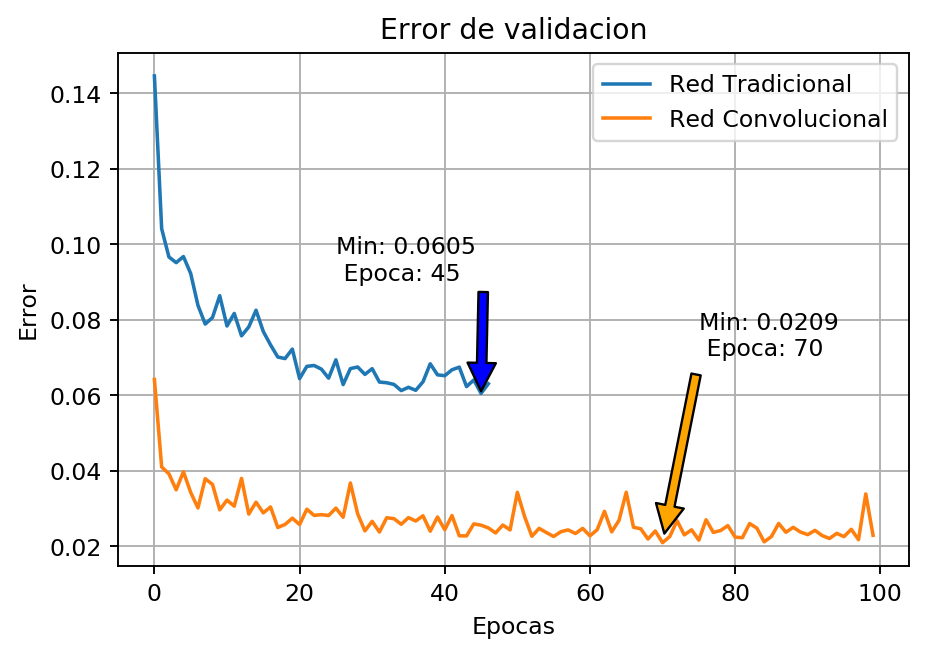
\includegraphics[width=0.75\textwidth]{img/valloss}
            \caption[Error de validación]{Error de validación. Fuente: Elaboración propia. }
            \label{fig:valloss}
        \end{figure}
        
        De manera similar al análisis de las curvas del error de entrenamiento se puede realizar algunas observaciones concernientes
        a las curvas del error de validación:

        \begin{itemize}
            \item \textbf{El error de inicial es menor:} Es un indicativo que la capacidad de generalización de la red convolucional 
            es mucho mayor desde la primera época. Es decir, que con solamente una pasada por el conjunto de entrenamiento, tiene una 
            capacidad mayor de realizar predicciones cercanas a la realidad en casos nunca antes vistos, como son las muestras del
            conjunto de validación.
            \item \textbf{El error mínimo es menor:} En este caso, el error de validación mínimo indica que la capacidad de generalización 
            de la red convolucional es mayor al de la red tradicional. Si el error de la red convolucional fuera mayor, esto podría indicar 
            sobreentrenamiento de la red. En este caso, se puede observar que se llega al mínimo alrededor de la época número 70.
            \item \textbf{Convergencia:} La convergencia del error de validación indica que ambas redes neuronales no están siendo 
            sobreentrenadas, sin embargo, los valores del error son menores para la red convolucional mostrando que su rendimiento 
            y capacidad de generalización son mayores al de una red tradicional.
        \end{itemize}
    
    \subsection{Puntajes y errores en el conjunto de prueba}\label{sec:scores}
    Más allá del análisis de las curvas de entrenamiento, se puede evaluar al modelo entrenado en base a sus puntajes o 
    \textit{scores} definidos para este tipo de tarea. En el presente proyecto, se evaluó a los modelos en base a 
    los puntajes definidos en la Tabla(\ref{tbl:metrics}).


    % Please add the following required packages to your document preamble:
    % \usepackage{booktabs}
    % \usepackage{graphicx}
    \begin{table}[!h]
        \centering
        \resizebox{0.65\textwidth}{!}{%
        \begin{tabular}{@{}|c|c|c|@{}}
        \toprule
        \textbf{Métrica} & \textbf{Nombre} & \textbf{Definición} \\ \midrule
        MSE & Error Cuadrático Medio & Ecuación(\ref{eq:mse}) \\ \midrule
        MAE & Error Absoluto Medio & Ecuación(\ref{eq:mae}) \\ \midrule
        $R^2$ & Coeficiente de Determinación & Ecuación(\ref{eq:r2}) \\ \bottomrule
        \end{tabular}%
        }
        \caption[Métricas para la evaluación del modelo.]{Métricas para la evaluación del modelo. Fuente: Elaboración propia.}
        \label{tbl:metrics}
    \end{table}

    Los resultados de la evaluación del modelo sobre el conjunto de prueba se pueden observar en la Tabla(\ref{tbl:testscores}) donde se 
    nota claramente la superioridad en todas las métricas de la red neuronal convolucional. 

    % Please add the following required packages to your document preamble:
    % \usepackage{booktabs}
    % \usepackage{graphicx}
    \begin{table}[!h]
        \centering
        \resizebox{0.45\textwidth}{!}{%
        \begin{tabular}{@{}|c|c|c|c|@{}}
        \toprule
        \textbf{Modelo} & \textbf{MSE} & \textbf{MAE} & $\mathbf{R^2}$ \\ \midrule
        Tradicional & 0.0254 & 0.0976 & 0.9278 \\ \midrule
        Convolucional & 0.0160 & 0.0872 & 0.9484 \\ \bottomrule
        \end{tabular}%
        }
        \caption[Evaluación de puntajes sobre el conjunto de prueba.]{Evaluación de puntajes sobre el conjunto de prueba. Fuente: Elaboración propia.}
        \label{tbl:testscores}
    \end{table}

    Se puede observar en detalle algunas predicciones en la Tabla(\ref{tbl:predsample}), de la cual se debe rescatar principalmente el signo 
    de la predicción que indica la dirección de viraje correcta.

    % Please add the following required packages to your document preamble:
    % \usepackage{booktabs}
    % \usepackage{graphicx}
    \begin{table}[]
        \centering
        \resizebox{0.55\textwidth}{!}{%
        \begin{tabular}{@{}|c|c|c|c|@{}}
        \toprule
        \textbf{Valor real} & \textbf{Predicción} & \textbf{Diferencia} & \textbf{\begin{tabular}[c]{@{}c@{}}Predicción de\\ signo correcta\end{tabular}} \\ \midrule
        -0.297 & -0.243 & 0.054 & \checkmark \\ \midrule
        1.0 & 0.921 & 0.079 & \checkmark \\ \midrule
        0.149 & 0.22 & 0.07 & \checkmark \\ \midrule
        -1. & -0.968 & 0.032 & \checkmark \\ \midrule
        -0. & 0.069 & 0.069 & $\times$ \\ \bottomrule
        \end{tabular}%
        }
        \caption[Muestra de predicciones de la red convolucional.]{Muestra de predicciones de la red convolucional. Fuente: Elaboración propia.}
        \label{tbl:predsample}
    \end{table}

    Nótese que la única predicción errónea en dirección de la muestra tiene que ver con un valor nulo, sin embargo, el error 
    de la predicción es muy similar a las otras muestras.
\section{Pruebas}\label{sec:analisistest}

Pese a que se ha validado la efectividad de la red neurona convolucional analizando el error en los conjuntos de entrenamiento, 
validación y prueba, es necesario realizar un análisis cualitativo de los resultados en base a pruebas de campo del modelo.
Se procede a analizar el rendimiento y generación de representaciones internas de la red neuronal convolucional dadas 
nuevas muestras que ingresan al modelo. Se presta especial atención al signo de la predicción.

    \subsection{Análisis del rendimiento en pruebas de campo}
    Dada la naturaleza de la tarea, es importante analizar de manera detallada las predicciones que está arrojando la red 
    neuronal para casos nuevos. Se ha grabado una nueva sesión de muestras para evaluar el rendimiento del sistema. Los 
    resultados de esta evaluación se pueden observar en la Figura(\ref{fig:testimg}).

    \begin{figure}[!h] 
        \centering
        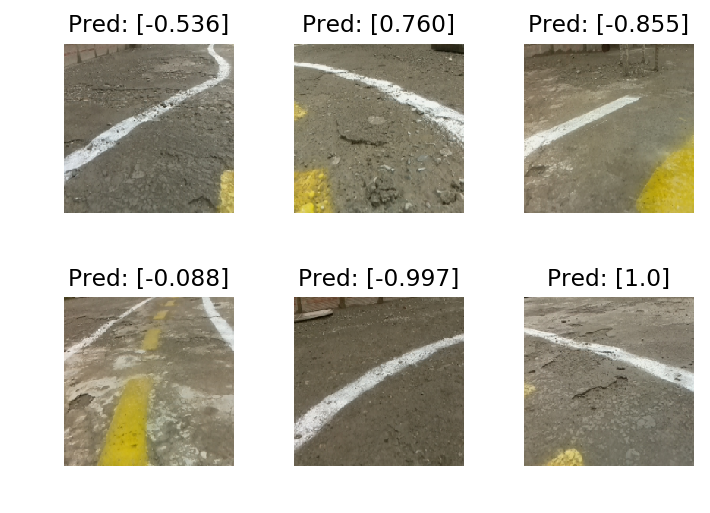
\includegraphics[width=0.75\textwidth]{img/testimg}
        \caption[Ejemplos de predicción de la red convolucional]{Ejemplos de predicción de la red convolucional. Fuente: Elaboración propia. }
        \label{fig:testimg}
    \end{figure}

    De la anterior figura, es importante tomar en cuenta que el signo de la predicción indica la dirección en la que se debe 
    mover el vehículo dada la imagen de la carretera. El signo correcto de la predicción es fundamental para el funcionamiento 
    adecuado del sistema. Una predición con signo errado puede llevar a la inestabilidad del sistema. 

    También se puede notar que la predicción es correcta pese a que no se puedan observar ambas líneas delimitadoras del carril 
    e incluso, en casos en los que la línea no cruza completamente la imagen.

    \subsection{Análisis de representaciones internas}\label{sec:representaciones}

    Ya se ha discutido la importancia de las capas convolucionales para la generación automática de representaciones internas 
    de los datos de entrada. En la Figura(\ref{fig:filtros1}) se puede visualizar los filtros de la primera capa convolucional.
    
    \begin{figure}[!h] 
        \centering
        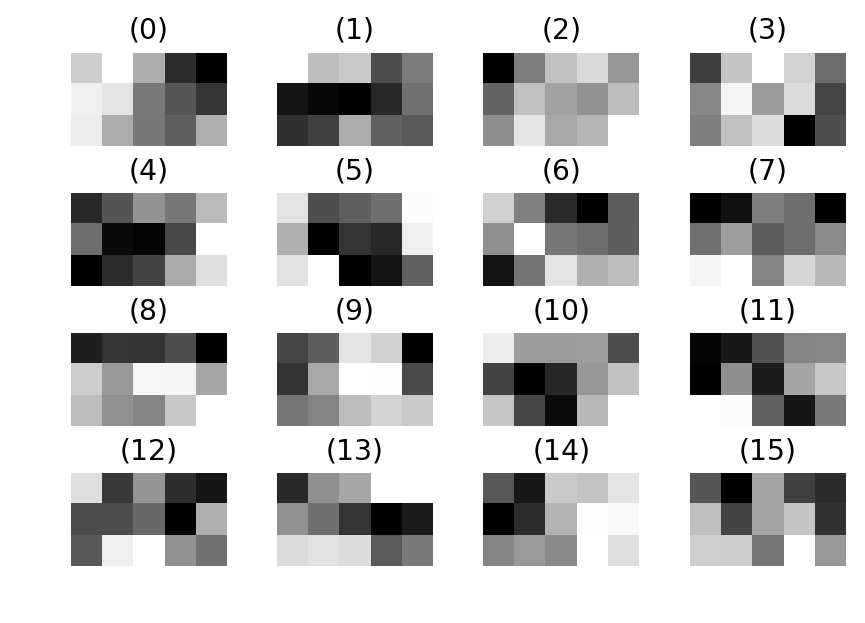
\includegraphics[width=0.65\textwidth]{img/filtros1}
        \caption[Filtros de la primera capa convolucional]{Filtros de la primera capa convolucional. Fuente: Elaboración propia. }
        \label{fig:filtros1}
    \end{figure}

    Es interesante analizar la naturaleza de los filtros generados en el proceso de aprendizaje. Por ejemplo, en el filtro 
    (\ref{fig:filtros1},0), se puede apreciar claramente que el filtro está dando importancia a bordes con una inclinación 
    hacia la derecha, de manera similar, el filtro (\ref{fig:filtros1},5) detecta bordes inclinados hacia la izquierda.

    
    \begin{figure}[!h] 
        \centering
        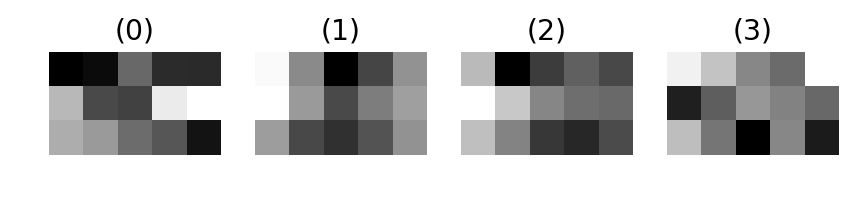
\includegraphics[width=0.65\textwidth]{img/filtros7}
        \caption[Filtros de la penúltima capa convolucional]{Filtros de la penúltima capa convolucional. Fuente: Elaboración propia. }
        \label{fig:filtros7}
    \end{figure}

    En el caso de los filtros de las capas superiores, se puede observar que las representaciones son mucho más abstractas. Por 
    ejemplo, en el filtro (\ref{fig:filtros7},0) se da importancia a activaciones que aparezcan a la derecna, en el 
    (\ref{fig:filtros7},2) a la izquierda y en el (\ref{fig:filtros7},4) a activaciones que aparecen a ambos lados, cuando 
    el vehículo está centrado en la carretera.

    Lo más importante en este análisis es resaltar el hecho de que la red neuronal ha generado estos filtros exclusivamente 
    mediante el proceso de aprendizaje basado en retropropagación de manera automática. En ningún momento en la etapa de diseño, 
    se ha incorporado algún criterio indicando que las líneas de la carretera tendrían bordes inclinados a la izquierda o derecha 
    o aparecerían a los costados de la imagen. Esto demuestra la impresionante capacidad de las redes neuronales convolucionales 
    para analizar imágenes de manera natural.

    Posteriormente, se puede analizar las activaciones que generan en las capas convolucionales algunas imágenes obtenidas 
    en la etapa de pruebas del prototipo. Se analizarán tres casos en los que la red establezca predicciones de 
    viraje a la izquierda, a la derecha y al centro.

        \subsubsection{Giro a la izquierda}
        En la Figura(\ref{fig:predizq}) se puede observar el paso de una imagen en la que el vehículo tiene que virar hacia la izquierda por 
        las capas convolucionales de la red neuronal. 

        \begin{figure}[!h] 
            \centering
            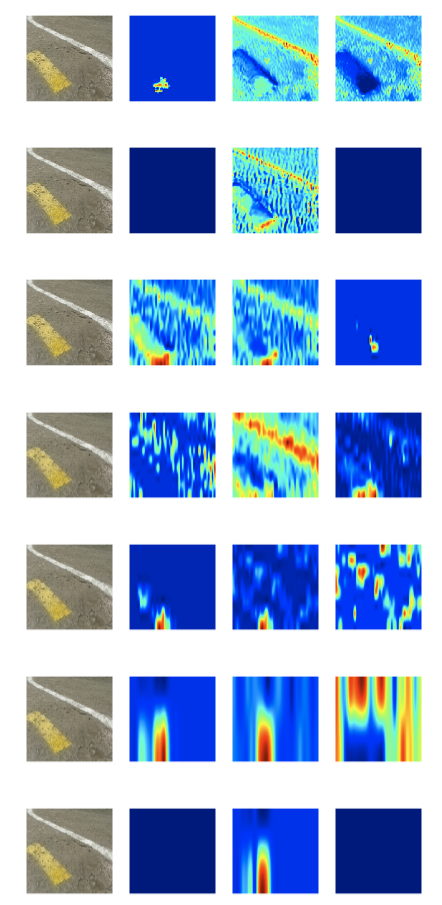
\includegraphics[width=0.60\textwidth]{img/predizq}
            \caption[Activaciones para una imagen con giro a la izquierda]{Activaciones para una imagen con giro a la izquierda, el valor de 
            la predicción es 1. Fuente: Elaboración propia. }
            \label{fig:predizq}
        \end{figure}

        Los mapas de características generados para esta imagen denotan activaciones con valor alto en las regiones donde estan 
        presentes las líneas de la carretera. A medida que se avanza en las capas convolucionales, se puede observar un máximo 
        en el lado izquierdo de la imagen. Este máximo corresponde con el valor de la predicción que se puede interpretar como un comando 
        de viraje máximo a la izquierda.
        

        \subsubsection{Giro a la derecha}
        En la Figura(\ref{fig:predder}) se puede observar el paso de una imagen en la que el vehículo tiene que virar hacia la derecha por 
        las capas convolucionales de la red neuronal. 

        \begin{figure}[!h] 
            \centering
            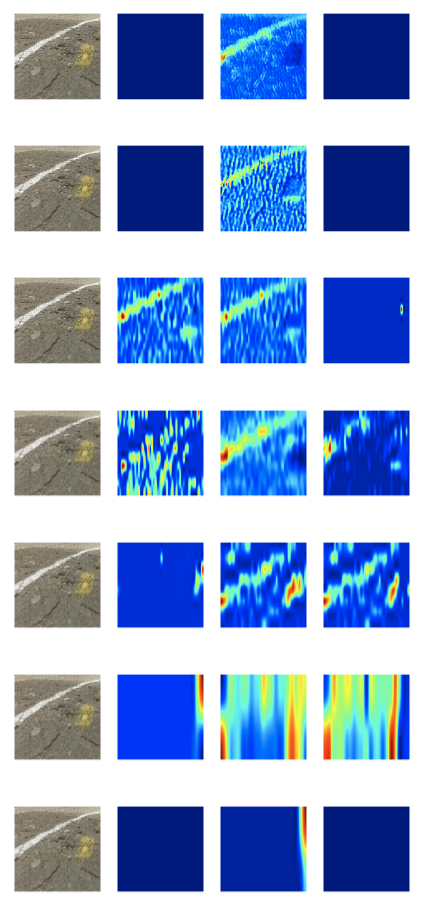
\includegraphics[width=0.60\textwidth]{img/predder}
            \caption[Activaciones para una imagen con giro a la derecha]{Activaciones para una imagen con giro a la derecha, el valor de 
            la predicción es -0.84. Fuente: Elaboración propia. }
            \label{fig:predder}
        \end{figure}

        Los mapas de características generados para esta imagen denotan activaciones con valor alto en las regiones donde estan 
        presentes las líneas de la carretera. A medida que se avanza en las capas convolucionales, se puede observar un máximo 
        en el lado derecho de la imagen. Este máximo corresponde con el valor de la predicción que se puede interpretar como un comando 
        de viraje a la derecha.


        \subsubsection{Conducir hacia adelante}
        En el caso en el que el vehículo se encuentre centrado, el comando de control debe aproximarse a cero, pues este 
        valor representa que se tiene que mantener la dirección actual. En la Figura(\ref{fig:predade}) se observa cómo el máximo se encuentra 
        cerca al centro de la imagen, lo que significa que el vehículo debe mantener su dirección. 


        \begin{figure}[!h] 
            \centering
            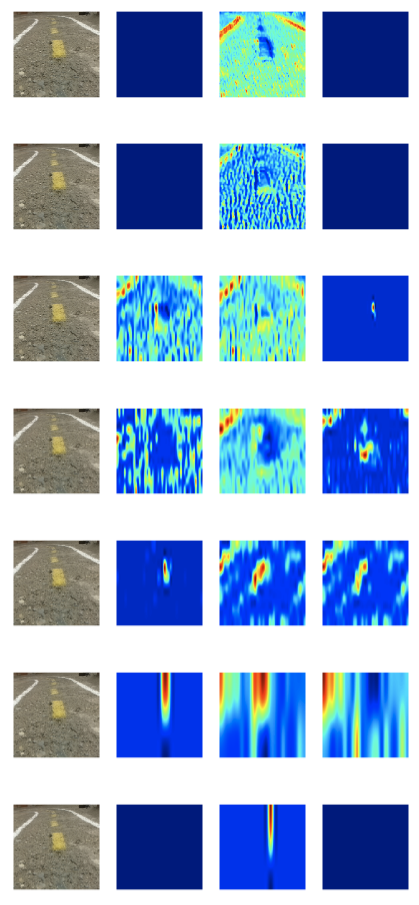
\includegraphics[width=0.60\textwidth]{img/predade}
            \caption[Activaciones para una imagen con dirección hacia adelante]{Activaciones para una imagen con dirección hacia adelante, el valor de 
            la predicción es -0.1. Fuente: Elaboración propia. }
            \label{fig:predade}
        \end{figure}

        De esta manera se ha podido observar la naturaleza del procesamiento que es capaz de hacer una red neuronal convolucional 
        y la forma en la que las representaciones internas que se generan en el aprendizaje son válidas para la 
        tarea de regresión.

